%% ============================================================ 1 PERMUTATIONS AND COMBINATIONS
\clearpage
\inchap{Permutations and Combinations}
\section{Counting Principles and Formulae}
\begin{center}\ba\small
\begin{tabular}{|M{3.4cm}|M{5.6cm}|M{6.2cm}|}\hline
 & \textbf{Addition principle} & \textbf{Multiplication principle}\\\Xhline{2pt}
Use when & either event $A$ \textbf{or} $B$ (cases) & stage 1 \textbf{and} stage 2 (steps)\\\hline
Condition & cases cannot happen together & stages are done one after another\\\hline
Total & $m+n$ & $m\times n$\\\hline
\end{tabular}\end{center}
\begin{center}\renewcommand{\arraystretch}{1.5}\small
\begin{tabular}{|M{3.1cm}|M{3.4cm}|M{4.8cm}|M{3.4cm}|}\hline
\textbf{Situation} & \textbf{Formula} & \textbf{Visual} & \textbf{Note}\\\Xhline{2pt}
$n$ distinct objects in a row & $n!$ & 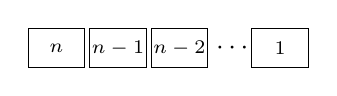
\begin{tikzpicture}[baseline=(current bounding box.center)]\node[draw,fill=white,minimum width=0.72cm,minimum height=0.5cm,inner sep=0pt,font=\scriptsize] at (0.36,0){$n$};\node[draw,fill=white,minimum width=0.72cm,minimum height=0.5cm,inner sep=0pt,font=\scriptsize] at (1.14,0){$n-1$};\node[draw,fill=white,minimum width=0.72cm,minimum height=0.5cm,inner sep=0pt,font=\scriptsize] at (1.92,0){$n-2$};\node at (2.59,0){$\cdots$};\node[draw,fill=white,minimum width=0.72cm,minimum height=0.5cm,inner sep=0pt,font=\scriptsize] at (3.20,0){$1$};\end{tikzpicture} & $0!=1$\\\hline
$r$ of $n$ distinct objects, in order & $\nCr{n}{r}\times r!=\dfrac{n!}{(n-r)!}$ & 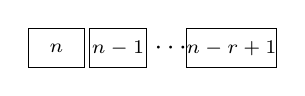
\begin{tikzpicture}[baseline=(current bounding box.center)]\node[draw,fill=white,minimum width=0.72cm,minimum height=0.5cm,inner sep=0pt,font=\scriptsize] at (0.36,0){$n$};\node[draw,fill=white,minimum width=0.72cm,minimum height=0.5cm,inner sep=0pt,font=\scriptsize] at (1.14,0){$n-1$};\node at (1.81,0){$\cdots$};\node[draw,fill=white,minimum width=1.05cm,minimum height=0.5cm,inner sep=0pt,font=\scriptsize] at (2.58,0){$n-r+1$};\end{tikzpicture} & order matters\\\hline
$r$ of $n$ distinct objects, no order & $\nCr{n}{r}=\dfrac{n!}{r!\,(n-r)!}$ & \rule{0pt}{0.75cm}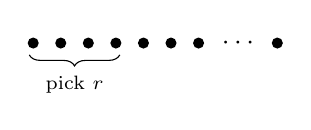
\begin{tikzpicture}[baseline=(current bounding box.center)]\fill (0.00,0) circle (2pt);\fill (0.35,0) circle (2pt);\fill (0.70,0) circle (2pt);\fill (1.05,0) circle (2pt);\fill (1.40,0) circle (2pt);\fill (1.75,0) circle (2pt);\fill (2.10,0) circle (2pt);\node at (2.6,0){$\cdots$};\fill (3.1,0) circle (2pt);\draw[decorate,decoration={brace,mirror,amplitude=4pt}] (-0.05,-0.15)--(1.1,-0.15) node[midway,below=4pt,font=\scriptsize]{pick $r$};\end{tikzpicture} & $\nCr{n}{r}=\nCr{n}{n-r}$\\\hline
$r$ places, each of $n$ choices, repeats allowed & $n^{r}$ & 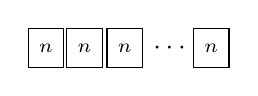
\begin{tikzpicture}[baseline=(current bounding box.center)]\node[draw,fill=white,minimum width=0.45cm,minimum height=0.5cm,inner sep=0pt,font=\scriptsize] at (0.23,0){$n$};\node[draw,fill=white,minimum width=0.45cm,minimum height=0.5cm,inner sep=0pt,font=\scriptsize] at (0.72,0){$n$};\node[draw,fill=white,minimum width=0.45cm,minimum height=0.5cm,inner sep=0pt,font=\scriptsize] at (1.23,0){$n$};\node at (1.80,0){$\cdots$};\node[draw,fill=white,minimum width=0.45cm,minimum height=0.5cm,inner sep=0pt,font=\scriptsize] at (2.33,0){$n$};\end{tikzpicture} & objects \textbf{can} be reused\\\hline
$n$ objects, $p$ alike of one kind, $q$ alike of another & $\dfrac{n!}{p!\,q!}$ & \rule{0pt}{0.8cm}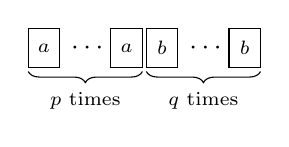
\begin{tikzpicture}[baseline=(current bounding box.center)]\node[draw,fill=white,minimum width=0.40cm,minimum height=0.5cm,inner sep=0pt,font=\scriptsize] at (0.20,0){$a$};\node at (0.75,0){$\cdots$};\node[draw,fill=white,minimum width=0.40cm,minimum height=0.5cm,inner sep=0pt,font=\scriptsize] at (1.25,0){$a$};\node[draw,fill=white,minimum width=0.40cm,minimum height=0.5cm,inner sep=0pt,font=\scriptsize] at (1.70,0){$b$};\node at (2.25,0){$\cdots$};\node[draw,fill=white,minimum width=0.40cm,minimum height=0.5cm,inner sep=0pt,font=\scriptsize] at (2.75,0){$b$};\draw[decorate,decoration={brace,mirror,amplitude=4pt}] (0,-0.3)--(1.45,-0.3) node[midway,below=4pt,font=\scriptsize]{$p$ times};\draw[decorate,decoration={brace,mirror,amplitude=4pt}] (1.5,-0.3)--(2.95,-0.3) node[midway,below=4pt,font=\scriptsize]{$q$ times};\end{tikzpicture} & divide by $k!$ for each $k$ identical\\\hline
$n$ distinct objects in a circle & $\dfrac{n!}{n}=(n-1)!$ & \rule{0pt}{0.75cm}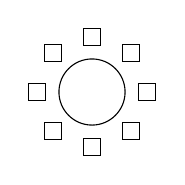
\begin{tikzpicture}[baseline=(current bounding box.center)]\draw (0,0) circle (0.42);\node[draw,rectangle,minimum width=0.22cm,minimum height=0.22cm,inner sep=0pt,font=\tiny] at (0.000,0.700){};\node[draw,rectangle,minimum width=0.22cm,minimum height=0.22cm,inner sep=0pt,font=\tiny] at (0.495,0.495){};\node[draw,rectangle,minimum width=0.22cm,minimum height=0.22cm,inner sep=0pt,font=\tiny] at (0.700,0.000){};\node[draw,rectangle,minimum width=0.22cm,minimum height=0.22cm,inner sep=0pt,font=\tiny] at (0.495,-0.495){};\node[draw,rectangle,minimum width=0.22cm,minimum height=0.22cm,inner sep=0pt,font=\tiny] at (0.000,-0.700){};\node[draw,rectangle,minimum width=0.22cm,minimum height=0.22cm,inner sep=0pt,font=\tiny] at (-0.495,-0.495){};\node[draw,rectangle,minimum width=0.22cm,minimum height=0.22cm,inner sep=0pt,font=\tiny] at (-0.700,-0.000){};\node[draw,rectangle,minimum width=0.22cm,minimum height=0.22cm,inner sep=0pt,font=\tiny] at (-0.495,0.495){};\end{tikzpicture} & rotations are the same\\\hline
\end{tabular}\end{center}
\gcs{\gc{nPr}, \gc{nCr}: \gckey{MATH} $\to$ \gc{PRB}. Type $n$ first, then the command, then $r$. \ \gc{!} is in the same menu.}
\begin{info}[title=Note]
Order matters $\Rightarrow$ select then arrange: $\nCr{n}{r}\times r!$
\end{info}
\section{Arrangements in a Line}
\begin{center}\ba\small
\begin{tabular}{|L{2.9cm}|L{4.1cm}|M{3.4cm}|M{4.2cm}|}\hline
\textbf{Condition} & \textbf{Method} & \textbf{Count} & \textbf{Visual}\\\Xhline{2pt}
Fixed position (e.g.\ $A$ first; number is even; first digit $\neq0$) & fill the restricted places \textbf{first}, then the rest & $\underline{\ k\ }\times\underline{\ \ }\times\cdots$ & \rule{0pt}{0.8cm}\begin{tikzpicture}[baseline=(current bounding box.center)]\node[draw,minimum width=0.42cm,minimum height=0.42cm,inner sep=0pt,font=\scriptsize] at (0.00,0){};\node[draw,minimum width=0.42cm,minimum height=0.42cm,inner sep=0pt,font=\scriptsize] at (0.50,0){};\node[draw,minimum width=0.42cm,minimum height=0.42cm,inner sep=0pt,font=\scriptsize] at (1.00,0){};\node at (1.5,0){$\cdots$};\node[draw,minimum width=0.42cm,minimum height=0.42cm,inner sep=0pt,font=\scriptsize] at (2.00,0){};\draw[-{Stealth},thick] (0,0.75)--(0,0.27);\end{tikzpicture}\\\hline
$A$, $B$ \textbf{together} & Grouping method: group $A$ and $B$ together, then arrange the blocks; arrange inside the block. & $(n-1)!\times2!$ & \rule{0pt}{0.8cm}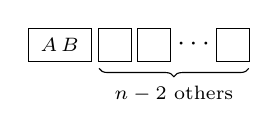
\begin{tikzpicture}[baseline=(current bounding box.center)]\node[draw,minimum width=0.8cm,minimum height=0.42cm,inner sep=0pt,font=\scriptsize] at (0.2,0){$A\,B$};\node[draw,minimum width=0.42cm,minimum height=0.42cm,inner sep=0pt,font=\scriptsize] at (0.90,0){};\node[draw,minimum width=0.42cm,minimum height=0.42cm,inner sep=0pt,font=\scriptsize] at (1.40,0){};\node at (1.9,0){$\cdots$};\node[draw,minimum width=0.42cm,minimum height=0.42cm,inner sep=0pt,font=\scriptsize] at (2.40,0){};\draw[decorate,decoration={brace,mirror,amplitude=3pt}] (0.7,-0.3)--(2.6,-0.3) node[midway,below=3pt,font=\scriptsize]{$n-2$ others};\end{tikzpicture}\\\hline
$A$, $B$ \textbf{separated} (complement) & total $-$ together & $n!-(n-1)!\,2!$ & \rule{0pt}{0.6cm}\scalebox{0.9}{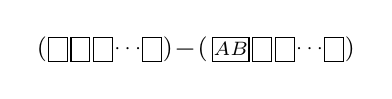
\begin{tikzpicture}[baseline=(current bounding box.center)]\node[font=\small] at (-0.20,0){$($};\node[draw,minimum width=0.24cm,minimum height=0.3cm,inner sep=0pt,font=\scriptsize] at (0.00,0){};\node[draw,minimum width=0.24cm,minimum height=0.3cm,inner sep=0pt,font=\scriptsize] at (0.29,0){};\node[draw,minimum width=0.24cm,minimum height=0.3cm,inner sep=0pt,font=\scriptsize] at (0.58,0){};\node[font=\scriptsize] at (0.89,0){$\cdots$};\node[draw,minimum width=0.24cm,minimum height=0.3cm,inner sep=0pt,font=\scriptsize] at (1.20,0){};\node[font=\small] at (1.40,0){$)$};\node at (1.62,0){$-$};\node[font=\small] at (1.84,0){$($};\node[draw,minimum width=0.46cm,minimum height=0.3cm,inner sep=0pt,font=\scriptsize] at (2.20,0){$AB$};\node[draw,minimum width=0.24cm,minimum height=0.3cm,inner sep=0pt,font=\scriptsize] at (2.60,0){};\node[draw,minimum width=0.24cm,minimum height=0.3cm,inner sep=0pt,font=\scriptsize] at (2.89,0){};\node[font=\scriptsize] at (3.2,0){$\cdots$};\node[draw,minimum width=0.24cm,minimum height=0.3cm,inner sep=0pt,font=\scriptsize] at (3.51,0){};\node[font=\small] at (3.71,0){$)$};\end{tikzpicture}}\\\hline
$A$, $B$ \textbf{separated} (slot in) & slot in: arrange the other $n-2$; choose 2 of the $n-1$ gaps for $A$, $B$; arrange $A$, $B$ & $(n-2)!\times\nCr{n-1}{2}\times2!$ & \rule{0pt}{0.9cm}\begin{tikzpicture}[baseline=(current bounding box.center)]\node[draw,minimum width=0.30cm,minimum height=0.32cm,inner sep=0pt,font=\scriptsize] at (0.20,0.00){};\node[draw,minimum width=0.30cm,minimum height=0.32cm,inner sep=0pt,font=\scriptsize] at (0.75,0.00){};\node[draw,minimum width=0.30cm,minimum height=0.32cm,inner sep=0pt,font=\scriptsize] at (1.30,0.00){};\node[draw,minimum width=0.30cm,minimum height=0.32cm,inner sep=0pt,font=\scriptsize] at (2.15,0.00){};\node[font=\scriptsize] at (1.73,0){$\cdots$};\draw[-{Stealth},thin] (-0.07,0.45)--(-0.07,0.2);\draw[-{Stealth},thin] (0.47,0.45)--(0.47,0.2);\draw[-{Stealth},thin] (1.02,0.45)--(1.02,0.2);\draw[-{Stealth},thin] (2.42,0.45)--(2.42,0.2);\node[draw,minimum width=0.30cm,minimum height=0.32cm,inner sep=0pt,font=\scriptsize] at (0.85,0.75){$A$};\node[draw,minimum width=0.30cm,minimum height=0.32cm,inner sep=0pt,font=\scriptsize] at (1.30,0.75){$B$};\node[font=\scriptsize,anchor=west] at (2.55,0){$n{-}1$ gaps};\end{tikzpicture}\\\hline
No two of a group adjacent & \textbf{slot in method}: arrange the other $m$; choose $k$ of the $m+1$ gaps for the group; arrange the group & $m!\times\nCr{m+1}{k}\times k!$ & \rule{0pt}{0.9cm}\begin{tikzpicture}[baseline=(current bounding box.center)]\node[draw,minimum width=0.30cm,minimum height=0.32cm,inner sep=0pt,font=\scriptsize] at (0.20,0.00){};\node[draw,minimum width=0.30cm,minimum height=0.32cm,inner sep=0pt,font=\scriptsize] at (0.75,0.00){};\node[draw,minimum width=0.30cm,minimum height=0.32cm,inner sep=0pt,font=\scriptsize] at (1.30,0.00){};\node[draw,minimum width=0.30cm,minimum height=0.32cm,inner sep=0pt,font=\scriptsize] at (2.15,0.00){};\node[font=\scriptsize] at (1.73,0){$\cdots$};\draw[-{Stealth},thin] (-0.07,0.45)--(-0.07,0.2);\draw[-{Stealth},thin] (0.47,0.45)--(0.47,0.2);\draw[-{Stealth},thin] (1.02,0.45)--(1.02,0.2);\draw[-{Stealth},thin] (2.42,0.45)--(2.42,0.2);\node[draw,minimum width=0.30cm,minimum height=0.32cm,inner sep=0pt,font=\scriptsize] at (0.85,0.75){$G$};\node[draw,minimum width=0.30cm,minimum height=0.32cm,inner sep=0pt,font=\scriptsize] at (1.30,0.75){$G$};\node[font=\scriptsize] at (1.75,0.75){$\cdots$};\node[font=\scriptsize,anchor=west] at (2.55,0){$m{+}1$ gaps};\end{tikzpicture}\\\hline
``at least one'' & complement: total $-$ none &  & \\\hline
$A$ \textbf{or} $B$ (or both) & add, then subtract the overlap once & $n(A)+n(B)-n(A\cap B)$ & \rule{0pt}{0.75cm}\vnn{white}{\sh}{\sh}{\sh}\\\hline
$A$ \textbf{or} $B$ but not both & add, then subtract the overlap twice & $n(A)+n(B)-2n(A\cap B)$ & \rule{0pt}{0.75cm}\vnn{white}{\sh}{\sh}{white}\\\hline
Several cases (e.g.\ last digit $0$ or not) & case table: count each case, then \textbf{add} &  & \\\hline
\end{tabular}\end{center}
\noindent\begin{minipage}[t]{0.48\textwidth}
\exlab Find the number of arrangements of the letters in the word STATISTICS.
\cdisp{\text{S}\times3,\ \text{T}\times3,\ \text{I}\times2\\\text{total}&=\dfrac{10!}{3!\,3!\,2!}\\&=50\,400}
\exlab Find the number of ways $4$ boys and $4$ girls can be arranged in a line such that boys and girls alternate.
\begin{center}\begin{tikzpicture}\node[draw,minimum width=0.42cm,minimum height=0.42cm,inner sep=0pt,font=\scriptsize,fill=blue!25] at (0.00,0.00){$B$};\node[draw,minimum width=0.42cm,minimum height=0.42cm,inner sep=0pt,font=\scriptsize,fill=blue!25] at (0.90,0.00){$B$};\node[draw,minimum width=0.42cm,minimum height=0.42cm,inner sep=0pt,font=\scriptsize,fill=blue!25] at (1.80,0.00){$B$};\node[draw,minimum width=0.42cm,minimum height=0.42cm,inner sep=0pt,font=\scriptsize,fill=blue!25] at (2.70,0.00){$B$};\draw[-{Stealth},red!75!black,thick] (-0.45,0.75)--(-0.45,0.25);\draw[-{Stealth},red!75!black,thick] (0.45,0.75)--(0.45,0.25);\draw[-{Stealth},red!75!black,thick] (1.35,0.75)--(1.35,0.25);\draw[-{Stealth},red!75!black,thick] (2.25,0.75)--(2.25,0.25);\draw[-{Stealth},black!45,thick] (0.45,-0.75)--(0.45,-0.25);\draw[-{Stealth},black!45,thick] (1.35,-0.75)--(1.35,-0.25);\draw[-{Stealth},black!45,thick] (2.25,-0.75)--(2.25,-0.25);\draw[-{Stealth},black!45,thick] (3.15,-0.75)--(3.15,-0.25);\end{tikzpicture}\end{center}
\cdisp{\text{total}&=2\times4!\times4!\\&=1152}
\end{minipage}\hfill
\begin{minipage}[t]{0.48\textwidth}
\exlab How many ways are there to arrange $6$ people in a line with $A$ and $B$ separated?
\begin{center}\begin{tikzpicture}\node[draw,minimum width=0.42cm,minimum height=0.42cm,inner sep=0pt,font=\scriptsize] at (0.00,0.00){};\node[draw,minimum width=0.42cm,minimum height=0.42cm,inner sep=0pt,font=\scriptsize] at (0.60,0.00){};\node[draw,minimum width=0.42cm,minimum height=0.42cm,inner sep=0pt,font=\scriptsize] at (1.20,0.00){};\node[draw,minimum width=0.42cm,minimum height=0.42cm,inner sep=0pt,font=\scriptsize] at (1.80,0.00){};\draw[-{Stealth},thin] (-0.30,0.55)--(-0.30,0.25);\draw[-{Stealth},thin] (0.30,0.55)--(0.30,0.25);\draw[-{Stealth},thin] (0.90,0.55)--(0.90,0.25);\draw[-{Stealth},thin] (1.50,0.55)--(1.50,0.25);\draw[-{Stealth},thin] (2.10,0.55)--(2.10,0.25);\node[draw,minimum width=0.42cm,minimum height=0.42cm,inner sep=0pt,font=\scriptsize] at (0.60,1.00){$A$};\node[draw,minimum width=0.42cm,minimum height=0.42cm,inner sep=0pt,font=\scriptsize] at (1.20,1.00){$B$};\end{tikzpicture}\end{center}
\cdisp{\text{total}&=4!\times\nCr{5}{2}\times2!\\&=480}
\exlab Even $3$-digit numbers from $0,1,2,3,4,5$, no repeats
\begin{center}\begin{tikzpicture}\node[draw,minimum width=0.42cm,minimum height=0.42cm,inner sep=0pt,font=\scriptsize] at (0.00,0.00){};\node[draw,minimum width=0.42cm,minimum height=0.42cm,inner sep=0pt,font=\scriptsize] at (0.55,0.00){};\node[draw,minimum width=0.42cm,minimum height=0.42cm,inner sep=0pt,font=\scriptsize] at (1.10,0.00){};\draw[-{Stealth},thick] (1.1,0.85)--(1.1,0.25);\node[font=\scriptsize,above] at (1.1,0.85){$0$};\node[font=\scriptsize,below] at (0.55,-0.25){Case 1};\end{tikzpicture}\qquad\begin{tikzpicture}\node[draw,minimum width=0.42cm,minimum height=0.42cm,inner sep=0pt,font=\scriptsize] at (0.00,0.00){};\node[draw,minimum width=0.42cm,minimum height=0.42cm,inner sep=0pt,font=\scriptsize] at (0.55,0.00){};\node[draw,minimum width=0.42cm,minimum height=0.42cm,inner sep=0pt,font=\scriptsize] at (1.10,0.00){};\draw[-{Stealth},thick] (1.1,0.85)--(1.1,0.25);\node[font=\scriptsize,above] at (1.1,0.85){$2,4$};\node[font=\scriptsize,below] at (0.55,-0.25){Case 2};\end{tikzpicture}\end{center}
\cdisp{\text{last }0&=5\times4=20\\\text{last }2\text{ or }4&=2\times4\times4=32\\\therefore\ \text{total}&=20+32\\&=52}
\end{minipage}
\section{Circular Arrangements}
\begin{center}\ba\small
\begin{tabular}{|L{2.9cm}|L{4.1cm}|M{3.4cm}|M{4.2cm}|}\hline
\textbf{Situation} & \textbf{Method} & \textbf{Count} & \textbf{Visual}\\\Xhline{2pt}
$n$ people round a table &  & $(n-1)!$ & \rule{0pt}{1.0cm}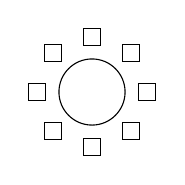
\begin{tikzpicture}[baseline=(current bounding box.center)]\draw (0,0) circle (0.42);\node[draw,rectangle,minimum width=0.22cm,minimum height=0.22cm,inner sep=0pt,font=\tiny] at (0.000,0.700){};\node[draw,rectangle,minimum width=0.22cm,minimum height=0.22cm,inner sep=0pt,font=\tiny] at (0.495,0.495){};\node[draw,rectangle,minimum width=0.22cm,minimum height=0.22cm,inner sep=0pt,font=\tiny] at (0.700,0.000){};\node[draw,rectangle,minimum width=0.22cm,minimum height=0.22cm,inner sep=0pt,font=\tiny] at (0.495,-0.495){};\node[draw,rectangle,minimum width=0.22cm,minimum height=0.22cm,inner sep=0pt,font=\tiny] at (0.000,-0.700){};\node[draw,rectangle,minimum width=0.22cm,minimum height=0.22cm,inner sep=0pt,font=\tiny] at (-0.495,-0.495){};\node[draw,rectangle,minimum width=0.22cm,minimum height=0.22cm,inner sep=0pt,font=\tiny] at (-0.700,-0.000){};\node[draw,rectangle,minimum width=0.22cm,minimum height=0.22cm,inner sep=0pt,font=\tiny] at (-0.495,0.495){};\end{tikzpicture}\\\hline
seats \textbf{numbered / distinguishable} & ignore the numbered seats and do everything as per normal, then multiply by the number of seats at the end & $(n-1)!\times n$ & \rule{0pt}{1.0cm}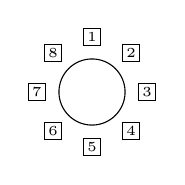
\begin{tikzpicture}[baseline=(current bounding box.center)]\draw (0,0) circle (0.42);\node[draw,rectangle,minimum width=0.22cm,minimum height=0.22cm,inner sep=0pt,font=\tiny] at (0.000,0.700){1};\node[draw,rectangle,minimum width=0.22cm,minimum height=0.22cm,inner sep=0pt,font=\tiny] at (0.495,0.495){2};\node[draw,rectangle,minimum width=0.22cm,minimum height=0.22cm,inner sep=0pt,font=\tiny] at (0.700,0.000){3};\node[draw,rectangle,minimum width=0.22cm,minimum height=0.22cm,inner sep=0pt,font=\tiny] at (0.495,-0.495){4};\node[draw,rectangle,minimum width=0.22cm,minimum height=0.22cm,inner sep=0pt,font=\tiny] at (0.000,-0.700){5};\node[draw,rectangle,minimum width=0.22cm,minimum height=0.22cm,inner sep=0pt,font=\tiny] at (-0.495,-0.495){6};\node[draw,rectangle,minimum width=0.22cm,minimum height=0.22cm,inner sep=0pt,font=\tiny] at (-0.700,-0.000){7};\node[draw,rectangle,minimum width=0.22cm,minimum height=0.22cm,inner sep=0pt,font=\tiny] at (-0.495,0.495){8};\end{tikzpicture}\\\hline
$A$, $B$ \textbf{together} & grouping, then circular arrangement of the blocks & $(n-2)!\times2!$ & \rule{0pt}{1.0cm}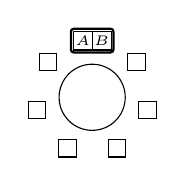
\begin{tikzpicture}[baseline=(current bounding box.center)]\draw (0,0) circle (0.42);\node[draw,rectangle,minimum width=0.24cm,minimum height=0.24cm,inner sep=0pt,font=\tiny] at (-0.120,0.720){$A$};\node[draw,rectangle,minimum width=0.24cm,minimum height=0.24cm,inner sep=0pt,font=\tiny] at (0.120,0.720){$B$};\draw[thick,rounded corners=1pt] (-0.27,0.570) rectangle (0.27,0.870);\node[draw,rectangle,minimum width=0.22cm,minimum height=0.22cm,inner sep=0pt,font=\tiny] at (0.563,0.449){};\node[draw,rectangle,minimum width=0.22cm,minimum height=0.22cm,inner sep=0pt,font=\tiny] at (0.702,-0.160){};\node[draw,rectangle,minimum width=0.22cm,minimum height=0.22cm,inner sep=0pt,font=\tiny] at (0.312,-0.649){};\node[draw,rectangle,minimum width=0.22cm,minimum height=0.22cm,inner sep=0pt,font=\tiny] at (-0.312,-0.649){};\node[draw,rectangle,minimum width=0.22cm,minimum height=0.22cm,inner sep=0pt,font=\tiny] at (-0.702,-0.160){};\node[draw,rectangle,minimum width=0.22cm,minimum height=0.22cm,inner sep=0pt,font=\tiny] at (-0.563,0.449){};\end{tikzpicture}\\\hline
$A$, $B$ \textbf{separated} (complement) & total $-$ together & $(n-1)!-(n-2)!\times2!$ & \rule{0pt}{1.0cm}\scalebox{0.68}{\begin{tikzpicture}[baseline=(current bounding box.center)]\node at (-1.6,0){\begin{tikzpicture}[baseline=(current bounding box.center)]\node[font=\large] at (-1.05,0){$($};\draw (0,0) circle (0.42);\node[draw,rectangle,minimum width=0.22cm,minimum height=0.22cm,inner sep=0pt,font=\tiny] at (0.000,0.700){};\node[draw,rectangle,minimum width=0.22cm,minimum height=0.22cm,inner sep=0pt,font=\tiny] at (0.495,0.495){};\node[draw,rectangle,minimum width=0.22cm,minimum height=0.22cm,inner sep=0pt,font=\tiny] at (0.700,0.000){};\node[draw,rectangle,minimum width=0.22cm,minimum height=0.22cm,inner sep=0pt,font=\tiny] at (0.495,-0.495){};\node[draw,rectangle,minimum width=0.22cm,minimum height=0.22cm,inner sep=0pt,font=\tiny] at (0.000,-0.700){};\node[draw,rectangle,minimum width=0.22cm,minimum height=0.22cm,inner sep=0pt,font=\tiny] at (-0.495,-0.495){};\node[draw,rectangle,minimum width=0.22cm,minimum height=0.22cm,inner sep=0pt,font=\tiny] at (-0.700,-0.000){};\node[draw,rectangle,minimum width=0.22cm,minimum height=0.22cm,inner sep=0pt,font=\tiny] at (-0.495,0.495){};\node[font=\large] at (1.05,0){$)$};\end{tikzpicture}};\node at (0,0){$-$};\node at (1.6,0){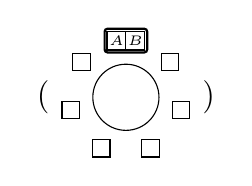
\begin{tikzpicture}[baseline=(current bounding box.center)]\node[font=\large] at (-1.05,0){$($};\draw (0,0) circle (0.42);\node[draw,rectangle,minimum width=0.24cm,minimum height=0.24cm,inner sep=0pt,font=\tiny] at (-0.120,0.720){$A$};\node[draw,rectangle,minimum width=0.24cm,minimum height=0.24cm,inner sep=0pt,font=\tiny] at (0.120,0.720){$B$};\draw[thick,rounded corners=1pt] (-0.27,0.570) rectangle (0.27,0.870);\node[draw,rectangle,minimum width=0.22cm,minimum height=0.22cm,inner sep=0pt,font=\tiny] at (0.563,0.449){};\node[draw,rectangle,minimum width=0.22cm,minimum height=0.22cm,inner sep=0pt,font=\tiny] at (0.702,-0.160){};\node[draw,rectangle,minimum width=0.22cm,minimum height=0.22cm,inner sep=0pt,font=\tiny] at (0.312,-0.649){};\node[draw,rectangle,minimum width=0.22cm,minimum height=0.22cm,inner sep=0pt,font=\tiny] at (-0.312,-0.649){};\node[draw,rectangle,minimum width=0.22cm,minimum height=0.22cm,inner sep=0pt,font=\tiny] at (-0.702,-0.160){};\node[draw,rectangle,minimum width=0.22cm,minimum height=0.22cm,inner sep=0pt,font=\tiny] at (-0.563,0.449){};\node[font=\large] at (1.05,0){$)$};\end{tikzpicture}};\end{tikzpicture}}\\\hline
$A$, $B$ \textbf{separated} (slot in) & slot in: arrange the other $n-2$ in a circle; choose 2 of the $n-2$ gaps for $A$, $B$; arrange $A$, $B$ & $(n-3)!\times\nCr{n-2}{2}\times2!$ & \rule{0pt}{1.0cm}\begin{tikzpicture}[baseline=(current bounding box.center)]\draw (0,0) circle (0.42);\node[draw,rectangle,minimum width=0.22cm,minimum height=0.22cm,inner sep=0pt,font=\tiny] at (0.360,0.624){};\node[draw,rectangle,minimum width=0.22cm,minimum height=0.22cm,inner sep=0pt,font=\tiny] at (0.720,0.000){};\node[draw,rectangle,minimum width=0.22cm,minimum height=0.22cm,inner sep=0pt,font=\tiny] at (0.360,-0.624){};\node[draw,rectangle,minimum width=0.22cm,minimum height=0.22cm,inner sep=0pt,font=\tiny] at (-0.360,-0.624){};\node[draw,rectangle,minimum width=0.22cm,minimum height=0.22cm,inner sep=0pt,font=\tiny] at (-0.720,-0.000){};\node[draw,rectangle,minimum width=0.22cm,minimum height=0.22cm,inner sep=0pt,font=\tiny] at (-0.360,0.624){};\draw[-{Stealth},thin] (0.000,1.050)--(0.000,0.780);\draw[-{Stealth},thin] (0.909,0.525)--(0.675,0.390);\draw[-{Stealth},thin] (0.909,-0.525)--(0.675,-0.390);\draw[-{Stealth},thin] (0.000,-1.050)--(0.000,-0.780);\draw[-{Stealth},thin] (-0.909,-0.525)--(-0.675,-0.390);\draw[-{Stealth},thin] (-0.909,0.525)--(-0.675,0.390);\node[draw,rectangle,minimum width=0.24cm,minimum height=0.24cm,inner sep=0pt,font=\tiny] at (1.350,0.550){$A$};\node[draw,rectangle,minimum width=0.24cm,minimum height=0.24cm,inner sep=0pt,font=\tiny] at (1.650,0.550){$B$};\end{tikzpicture}\\\hline
$A$, $B$ in fixed relation (e.g.\ $A$ opposite $B$) & fix $A$; $B$ has 1 place; arrange the rest & $(n-2)!$ & \rule{0pt}{1.0cm}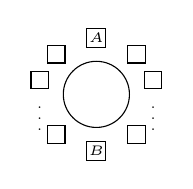
\begin{tikzpicture}[baseline=(current bounding box.center)]\draw (0,0) circle (0.42);\node[draw,rectangle,minimum width=0.24cm,minimum height=0.24cm,inner sep=0pt,font=\tiny] at (0.000,0.720){$A$};\node[draw,rectangle,minimum width=0.24cm,minimum height=0.24cm,inner sep=0pt,font=\tiny] at (0.000,-0.720){$B$};\node[draw,rectangle,minimum width=0.22cm,minimum height=0.22cm,inner sep=0pt,font=\tiny] at (0.509,0.509){};\node[draw,rectangle,minimum width=0.22cm,minimum height=0.22cm,inner sep=0pt,font=\tiny] at (0.509,-0.509){};\node[draw,rectangle,minimum width=0.22cm,minimum height=0.22cm,inner sep=0pt,font=\tiny] at (-0.509,0.509){};\node[draw,rectangle,minimum width=0.22cm,minimum height=0.22cm,inner sep=0pt,font=\tiny] at (-0.509,-0.509){};\node[draw,rectangle,minimum width=0.22cm,minimum height=0.22cm,inner sep=0pt,font=\tiny] at (0.720,0.180){};\node[draw,rectangle,minimum width=0.22cm,minimum height=0.22cm,inner sep=0pt,font=\tiny] at (-0.720,0.180){};\node[font=\tiny] at (0.72,-0.2){$\vdots$};\node[font=\tiny] at (-0.72,-0.2){$\vdots$};\end{tikzpicture}\\\hline
no two of $k$ people adjacent & \textbf{slot in method}: arrange the other $m$ in a circle; choose $k$ of the $m$ gaps; arrange the $k$ people & $(m-1)!\times\nCr{m}{k}\times k!$ & \rule{0pt}{1.0cm}\begin{tikzpicture}[baseline=(current bounding box.center)]\draw (0,0) circle (0.42);\node[draw,rectangle,minimum width=0.22cm,minimum height=0.22cm,inner sep=0pt,font=\tiny] at (0.360,0.624){};\node[draw,rectangle,minimum width=0.22cm,minimum height=0.22cm,inner sep=0pt,font=\tiny] at (0.720,0.000){};\node[draw,rectangle,minimum width=0.22cm,minimum height=0.22cm,inner sep=0pt,font=\tiny] at (0.360,-0.624){};\node[draw,rectangle,minimum width=0.22cm,minimum height=0.22cm,inner sep=0pt,font=\tiny] at (-0.360,-0.624){};\node[draw,rectangle,minimum width=0.22cm,minimum height=0.22cm,inner sep=0pt,font=\tiny] at (-0.720,-0.000){};\node[draw,rectangle,minimum width=0.22cm,minimum height=0.22cm,inner sep=0pt,font=\tiny] at (-0.360,0.624){};\draw[-{Stealth},thin] (0.000,1.050)--(0.000,0.780);\draw[-{Stealth},thin] (0.909,0.525)--(0.675,0.390);\draw[-{Stealth},thin] (0.909,-0.525)--(0.675,-0.390);\draw[-{Stealth},thin] (0.000,-1.050)--(0.000,-0.780);\draw[-{Stealth},thin] (-0.909,-0.525)--(-0.675,-0.390);\draw[-{Stealth},thin] (-0.909,0.525)--(-0.675,0.390);\node[draw,rectangle,minimum width=0.24cm,minimum height=0.24cm,inner sep=0pt,font=\tiny] at (1.350,0.550){$G$};\node[draw,rectangle,minimum width=0.24cm,minimum height=0.24cm,inner sep=0pt,font=\tiny] at (1.650,0.550){$G$};\node[font=\tiny] at (0.45,1.3){$\cdots$};\end{tikzpicture}\\\hline
\end{tabular}\end{center}
\section{Selections and Groups}
\begin{center}\renewcommand{\arraystretch}{1.0}\small
\begin{tabular}{|L{4.6cm}|L{6.4cm}|M{4.2cm}|}\hline
\textbf{Situation} & \textbf{Method} & \textbf{Count}\\\Xhline{2pt}
choose $r$ of $n$, with a condition (e.g.\ $\geq1$ woman) & $\nCr{n}{r}$; cases (add), or complement & total $-$ none\\\hline
choose, \textbf{then} arrange & select, then multiply by $r!$ (or by the arrangements) & $\nCr{n}{r}\times r!$\\\hline
``at least one of \textbf{each} kind'' & consider cases\newline Do \textbf{not} choose one of each first, then mix the rest together and choose the remaining (overcounts) & add cases\\\hline
forming words / codes with \textbf{repeated} letters & cases by the pattern of repeats (all different; one pair; \ldots): choose the letters, then arrange $\dfrac{r!}{p!\,q!}$ & add the cases\\\hline
groups of \textbf{different} sizes / labelled groups & choose group by group; named teams, different tasks or sizes: \textbf{no} division & $\nCr{n}{a}\,\nCr{n-a}{b}\cdots$\\\hline
$k$ groups of the \textbf{same} size, unlabelled & as above, then $\div\,k!$ (identical groups of equal size) & $\dfrac{\nCr{n}{a}\,\nCr{n-a}{a}\cdots}{k!}$\\\hline
\end{tabular}\end{center}
\noindent\begin{minipage}[t]{0.30\textwidth}
\exlab $8$ people into two groups of $4$
\cdisp{\text{unlabelled}&=\dfrac{\nCr{8}{4}}{2!}=35\\\text{teams }X,Y&=\nCr{8}{4}=70}
\end{minipage}\hfill
\begin{minipage}[t]{0.33\textwidth}
\exlab $3$-letter codes from MISSISSIPPI
\cdisp{\text{all different}&=\nCr{4}{3}\times3!=24\\\text{one pair}&=(3\times3)\times\dfrac{3!}{2!}=27\\\text{all alike}&=2\\\therefore\ \text{total}&=53}
\end{minipage}\hfill
\begin{minipage}[t]{0.33\textwidth}
\exlab $5$ from $3$ red, $4$ green, $5$ blue; every colour used
\cdisp{(3,1,1)&=\nCr{3}{3}\times\nCr{4}{1}\times\nCr{5}{1}=20\\(1,3,1)&=\nCr{3}{1}\times\nCr{4}{3}\times\nCr{5}{1}=60\\(1,1,3)&=\nCr{3}{1}\times\nCr{4}{1}\times\nCr{5}{3}=120\\(2,2,1)&=\nCr{3}{2}\times\nCr{4}{2}\times\nCr{5}{1}=90\\(2,1,2)&=\nCr{3}{2}\times\nCr{4}{1}\times\nCr{5}{2}=120\\(1,2,2)&=\nCr{3}{1}\times\nCr{4}{2}\times\nCr{5}{2}=180\\\therefore\ \text{ways}&=20+60+120\\&\quad+90+120+180\\&=590}
\end{minipage}
